\documentclass[12pt,a4paper]{report}
% Essential packages
\usepackage{natbib}
\usepackage[utf8]{inputenc}  
\usepackage[T1]{fontenc}
\usepackage{graphicx}
\usepackage{amsmath}
\usepackage{amsfonts}
\usepackage{amssymb}
\usepackage{fancyhdr}
\usepackage{xcolor}

% For Greek text support with XeLaTeX
\usepackage{fontspec}
\setmainfont{Times New Roman}
\newfontfamily\greekfont{Times New Roman}

% Page layout
\usepackage[margin=2.5cm]{geometry}
\usepackage{setspace}

% For better tables
\usepackage{booktabs}
\usepackage{array}

% For better lists
\usepackage{enumitem}

% For custom TOC formatting
\usepackage{tocloft}

% For section formatting
\usepackage{titlesec}

% Customize subsection formatting
\titleformat{\section}[hang]
  {\large\bfseries}  % Medium size (between chapter and subsection)
  {\thesection}
  {1em}
  {}
  []
\titlespacing*{\section}
  {0pt}     % left spacing
  {14pt}    % space before
  {7pt}     % space after

% For subsections (1.1.1, 1.1.2, etc.) - smaller size
\titleformat{\subsection}[hang]
  {\normalsize\bfseries}  % Smaller than sections
  {\thesubsection}
  {1em}
  {}
  []
\titlespacing*{\subsection}
  {0pt}     % left spacing
  {10pt}    % space before
  {5pt}     % space after

% For hyperlinks (load near the end)
\usepackage{hyperref}

% Set line spacing
\onehalfspacing

% Set up header height
\setlength{\headheight}{15pt}

% Add space between footnotes and main text
\addtolength{\skip\footins}{6pt}

% Configure hyperref
\hypersetup{
    colorlinks=true,
    linkcolor=black,
    filecolor=magenta,      
    urlcolor=blue,
    citecolor=black,
    pdftitle={Ars Post Faber},
    pdfauthor={Jorge Muñoz Zanón}
}

% Custom command for consistent title formatting (matching abstract style)
\newcommand{\formattedtitle}[1]{%
    \vspace{1cm}%
    \noindent%
    {\Large\textbf{#1}}%
    \vspace{0.3cm}%
    \hrule%
    \vspace{0.8cm}%
    \setlength{\parindent}{0pt}%
}

% Customize TOC title
\renewcommand{\contentsname}{}
\renewcommand{\cftaftertoctitle}{}
\renewcommand{\cftbeforetoctitleskip}{0pt}
\renewcommand{\cftaftertoctitleskip}{0pt}

% Customize LOF title
\renewcommand{\listfigurename}{}
\renewcommand{\cftafterloftitle}{}
\renewcommand{\cftbeforeloftitleskip}{0pt}
\renewcommand{\cftafterloftitleskip}{0pt}

% Customize LOT title
\renewcommand{\listtablename}{}
\renewcommand{\cftafterlottitle}{}
\renewcommand{\cftbeforelottitleskip}{0pt}
\renewcommand{\cftafterlottitleskip}{0pt}

% Bibliography formatting
\setlength{\bibsep}{6pt} % Space between bibliography entries
\setlength{\bibhang}{1.5em} % Hanging indent for bibliography entries

% Remove default bibliography title and spacing (we'll use custom formatting)
\renewcommand{\bibname}{}
\renewcommand{\refname}{}

% Remove extra space before bibliography
\makeatletter
\renewenvironment{thebibliography}[1]
     {\list{\@biblabel{\@arabic\c@enumiv}}%
           {\settowidth\labelwidth{\@biblabel{#1}}%
            \leftmargin\labelwidth
            \advance\leftmargin\labelsep
            \@openbib@code
            \usecounter{enumiv}%
            \let\p@enumiv\@empty
            \renewcommand\theenumiv{\@arabic\c@enumiv}}%
      \sloppy
      \clubpenalty4000
      \@clubpenalty \clubpenalty
      \widowpenalty4000%
      \sfcode`\.\@m}
     {\def\@noitemerr
       {\@latex@warning{Empty `thebibliography' environment}}%
      \endlist}
\makeatother
\begin{document}

% Title page
\begin{titlepage}
\centering
\vspace*{2.5cm}

% Title - Bold Italic
{\fontsize{24}{28}\selectfont\textbf{\textit{Ars Post Faber}}}

\vspace{0.3cm}

% Subtitle - Bold
{\fontsize{18}{22}\selectfont\textbf{Digital Fabrication democratization through embodied knowledge preservation}}

\vspace{0.4cm}

% Author line
{\fontsize{14}{16}\selectfont by}

\vspace{0.4cm}

% Author name - Italic
{\fontsize{16}{20}\selectfont\textit{Jorge Muñoz Zanón}}

\vspace{1.5cm}

% Thesis Advisors
{\fontsize{12}{15}\selectfont
\textbf{Thesis Advisors:}\\[0.1cm]
Jessica Carmen Guy\\
Roger Guilemany\\
Alejandra Tothill
}

\vspace{2cm}

% Institution and Program
{\fontsize{12}{15}\selectfont
Institute for Advanced Architecture of Catalonia (IAAC)\\[0.05cm]
Master in Design for Emergent Futures (MDEF) 2023 - 2025\\[0.05cm]
Thesis Cluster: MDEF02
}

\vspace{2cm}

% Location and Date
{\fontsize{14}{16}\selectfont Barcelona, Catalunya\\[0.05cm]
August 2025}

\vspace{3cm}

% Logos - side by side with Fab Lab bigger
\begin{center}

\includegraphics[height=1.2cm]{figures/logo/iaac_logo.pdf}
\hspace{1.5cm}

\includegraphics[height=1.6cm]{figures/logo/fablabbcn-logo.pdf}
\end{center}

\end{titlepage}

% Start page numbering with roman numerals for front matter
\pagenumbering{roman}
\setcounter{page}{1}

% Abstract on its own page (page i)
\newpage
% Header with advisor names
\noindent
\begin{minipage}[t]{0.5\textwidth}
\raggedright
Theiss Advisor: Jessica Carmen Guy
\end{minipage}%
\begin{minipage}[t]{0.5\textwidth}
\raggedleft
Jorge Muñoz Zanón
\end{minipage}
\vspace{1cm}

% Abstract title - left aligned with padding and underline
\noindent
{\Large\textbf{Abstract}}
\vspace{0.3cm}
\hrule
\vspace{0.8cm}

% Set no paragraph indentation for the abstract content
\setlength{\parindent}{0pt}

Digital fabrication technologies have democratized access to production tools while perpetuating the industrial era separation between design conception and material execution. This division, which has historically diminished artisanship by fragmenting holistic creative processes, continues to manifest itself in contemporary CAD/CAM workflows that benefit computational precision over embodied knowledge and tacit decision-making central to craftship, often reducing creation to pure geometry, failing to preserve the material relationships and adaptive responses that characterize traditional making practices.

\vspace{0.5cm}

This research challenges the assumption that fabrication democratization is achieved solely through access to scaled-down industrial tools and instead, looks out to do a reimagination of the relationship between maker, material, and technology, seeking to restore the holistic nature of creative practice within digital contexts, addressing how to preserve creative agency, embodied knowledge, and capacity for personal expression in digital fabrication contexts.

\vspace{0.5cm}

Through experimental tool testing and digital fabrication workshops with artisans and makers, this research develops \textit{Ars Post Faber}, an open-source Grasshopper plug-in within the Rhinoceros CAD environment that approaches thinking and making as an integrated practice. The plug-in implements utilities designed to facilitate fluid Human-Software-Machine interactions, looking to enable embodied expression, contextual adaptation, and tacit knowledge to flow throughout the making process. Rather than abstracting away the creative journey, this approach looks to preserve the complete narrative of creation, including modifications, errors, and decision points, as integral components of the final work.

\vspace{0.5cm}

By attempting to bridge the gap between digital design and material execution, this research looks to contribute to evolving discussions around craft, technology, and creative agency in the digital age, suggesting that true democratization might require representational frameworks that honor the complexity and continuity of human creative processes.

\vspace{1cm}

\noindent
\textbf{Keywords:} craftship, digital fabrication, human-machine interactions, preservation, democratization, artisanship

\vspace{\fill}

% Table of contents with custom formatting
\newpage
\formattedtitle{Contents}
\tableofcontents

% List of figures with custom formatting
\newpage
\formattedtitle{List of Figures}
\listoffigures

% List of tables with custom formatting
\newpage
\formattedtitle{List of Tables}
\listoftables

% Start main content with arabic numbering
\newpage
\pagenumbering{arabic}
\setcounter{page}{1}

% Main content sections 
% Set chapter counter to 1 and reset section counter
\setcounter{chapter}{1}
\setcounter{section}{0}

% Custom chapter title to match abstract formatting
\noindent
{\Large\textbf{Chapter 1: Introduction}}
\vspace{0.3cm}
\hrule
\vspace{0.8cm}
\label{ch:introduction}

% Set no paragraph indentation
\setlength{\parindent}{0pt}


        
\clearpage

\setcounter{chapter}{2}
\setcounter{section}{0}

% Add the chapter to table of contents
\addcontentsline{toc}{chapter}{\numberline{2}Rethinking Democratization: Beyond Access to Preservation}

\pagestyle{fancy}
\fancyhf{} % Clear all header and footer fields
\fancyhead[L]{\footnotesize\textit{Ars Post Faber: Digital Fabrication Democratization Through Embodied Knowledge Preservation}}
\fancyfoot[C]{\thepage} % Page number in footer center
\renewcommand{\headrulewidth}{0pt}
\renewcommand{\footrulewidth}{0pt}

\noindent
{\Large\textbf{Chapter 2: Rethinking Democratization: Beyond Access to Preservation}}
\vspace{0.3cm}
\hrule
\vspace{0.8cm}
\label{ch:democratization}

% Set no paragraph indentation
\setlength{\parindent}{0pt}

The historical trajectory examined in Chapter 1 has showed how creative agency has been systematically redistributed from unified practice to contemporary digital workflows. This analysis raises the question: if digital fabrication technologies possess unprecedented capabilities for material manipulation and geometric exploration, why do they continue to perpetuate the same distributed agency frameworks that eliminated adaptive authority? The answer lies in how the "democratization" itself has been conceptualized within digital fabrication discourse.

\vspace{0.5cm}

Rather than addressing the organizational structures that fragment creative agency, contemporary digital fabrication has pursued democratization primarily through expanded access to scaled-down industrial tools. This chapter will examine how this access-centered approach, while achieving remarkable quantitative success, fails to address the deeper structural issues identified in the historical analysis. By tracing the evolution from access-based democratization toward preservation-centered approaches, this chapter will try to pursue a reconceptualization of what democratic making might mean in digital contexts.

\section{The Access Paradigm and Its Achievements}

This access-centered understanding of democratization has become the dominant paradigm within contemporary digital fabrication discourse. Neil Gershenfeld's\footnote{Neil Gershenfeld is a physicist at MIT who's the director of the Center for Bits and Atoms (CBA) and pioneered the global FabLab movement. His work focuses on the intersection of physical and digital systems, advocating for "personal fabrication" as a means to democratize access to manufacturing capabilities.} foundational vision for FabLabs\footnote{FabLabs (Fabrication Laboratories) are digital fabrication workshops that provide public access to tools for invention, prototyping and local production. Originally conceived at MIT's Center for Bits and Atoms, FabLabs follow a global charter emphasizing open access, education, and local innovation while connecting to a worldwide network of collaborative spaces.} promised "personal fabrication" enabling "almost anyone to make almost anything" \citep{gershenfeld2007}, positioning digital fabrication as the natural evolution of personal computing—bringing the same accessibility that desktop computers brought to information processing into the realm of physical manufacturing. This vision emphasized scaling down industrial production capabilities to individual users, making sophisticated fabrication tools available in community workshops and educational institutions.

\vspace{0.5cm}

\begin{figure}[h]
\centering
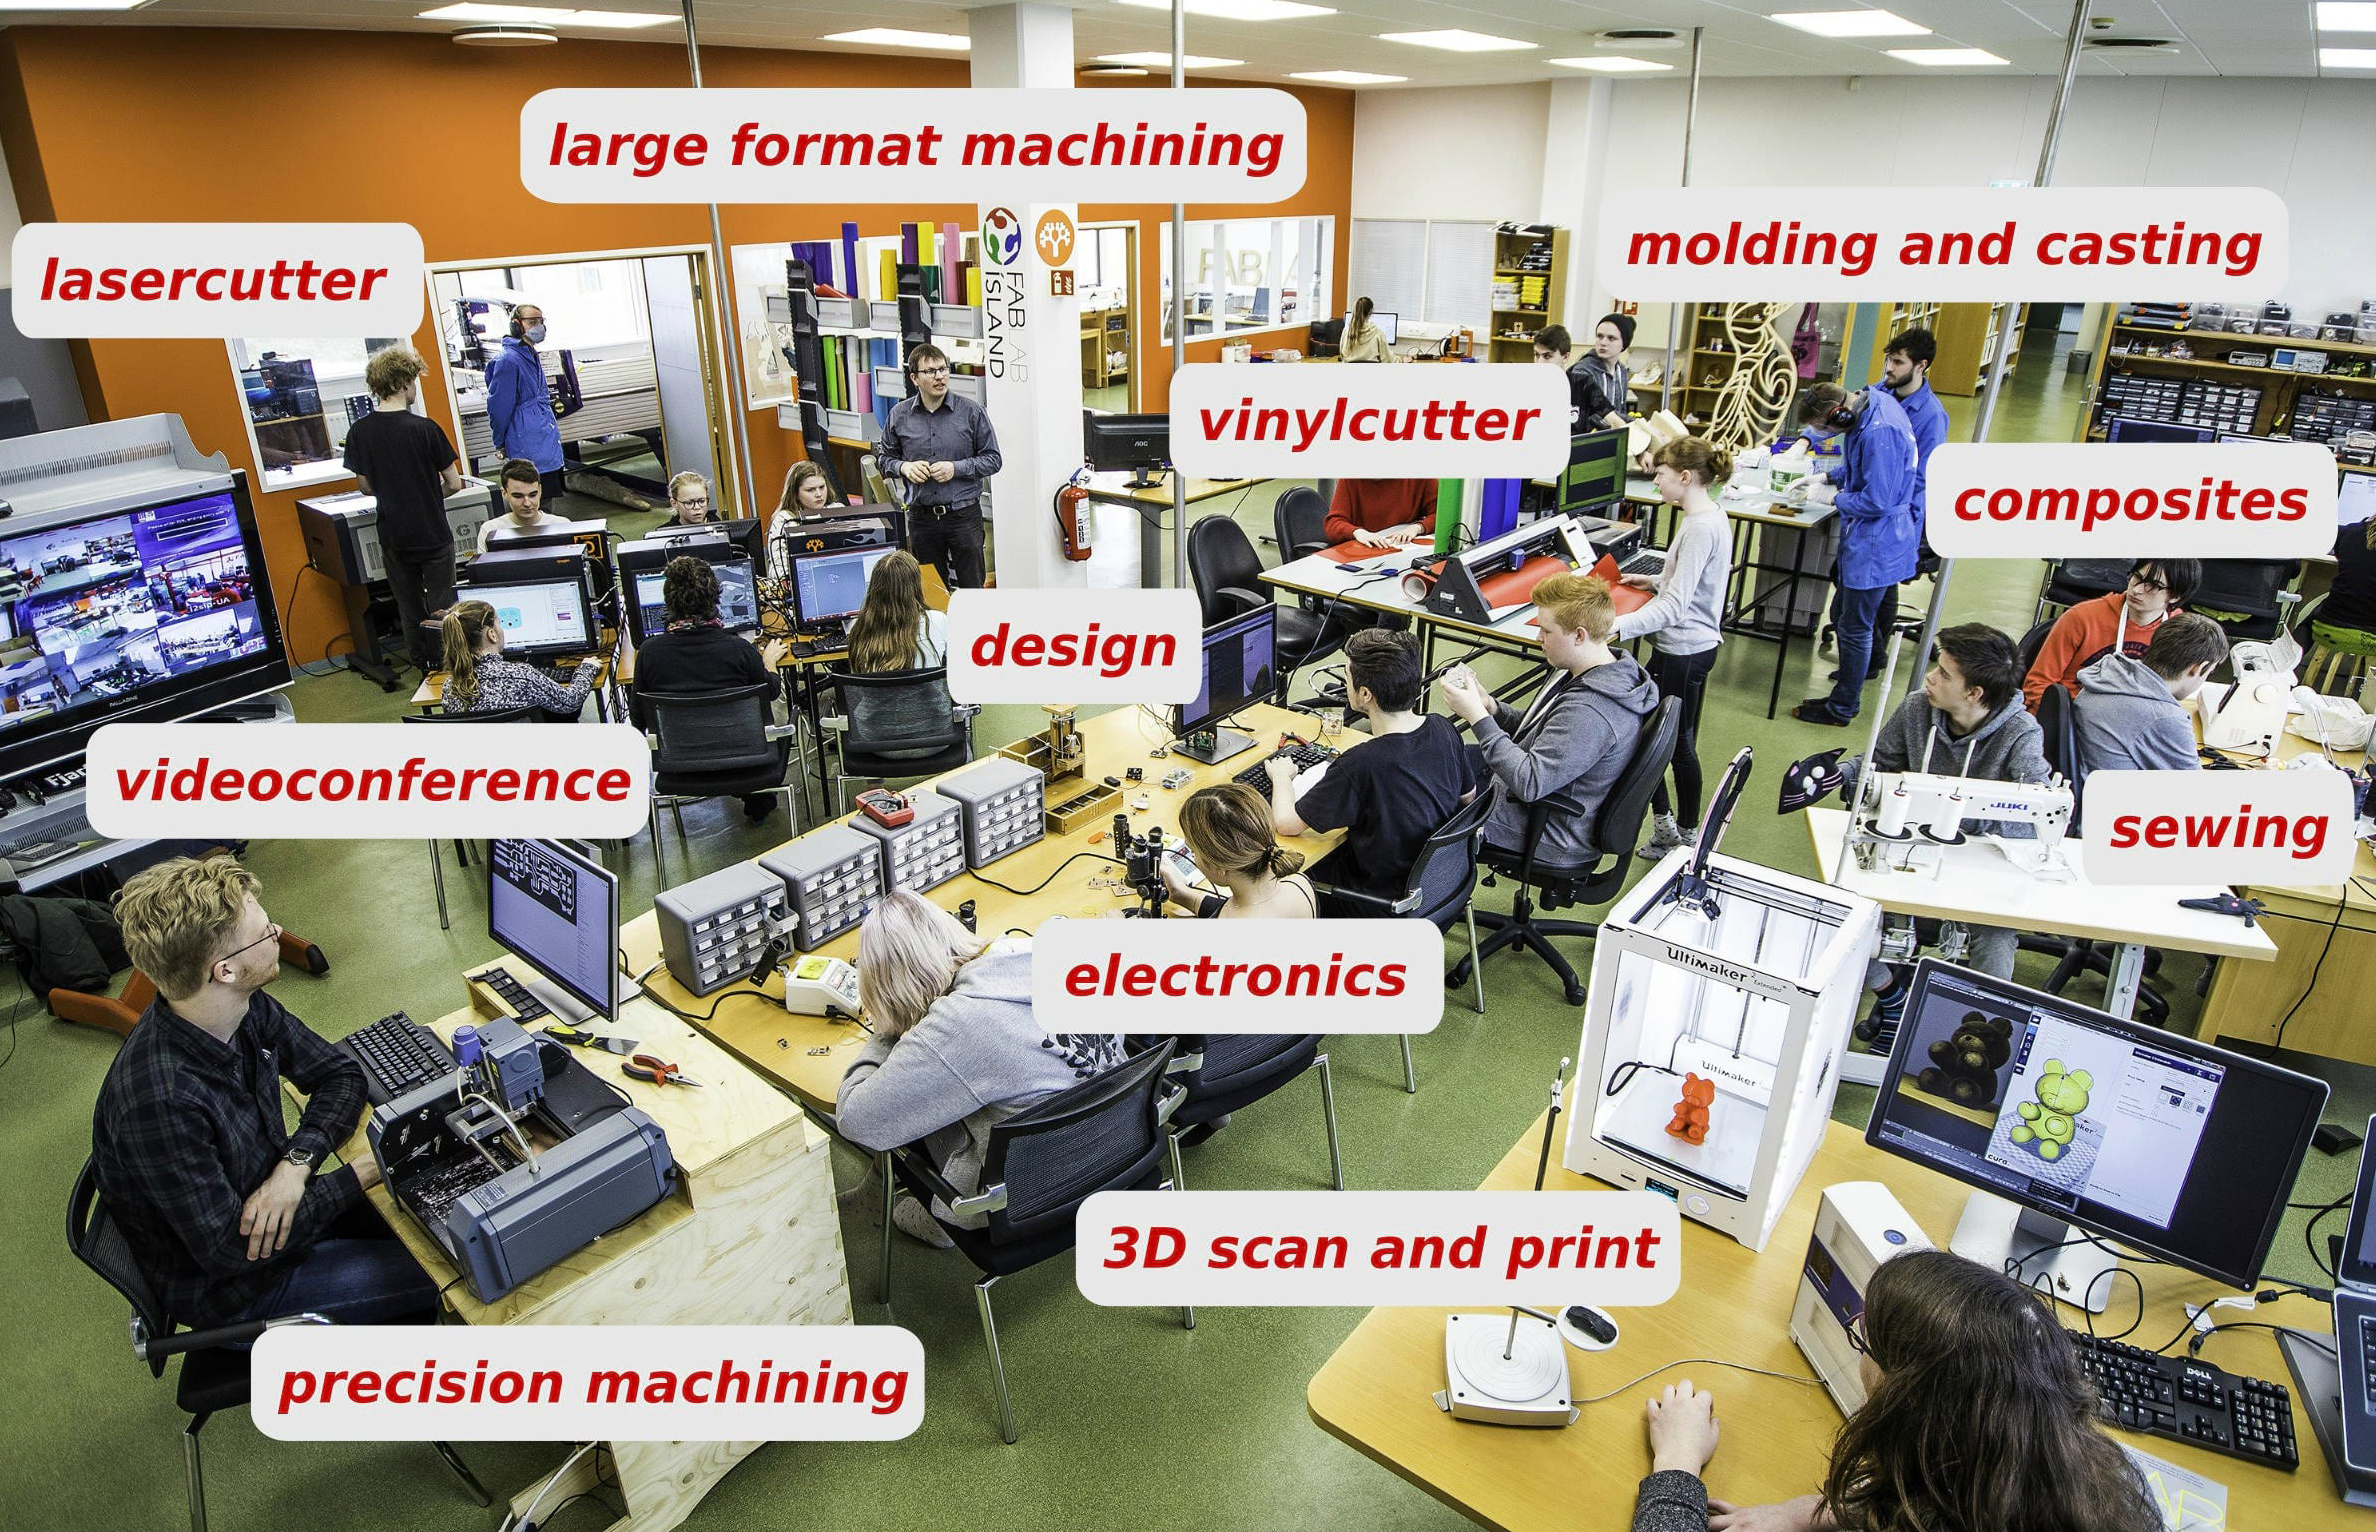
\includegraphics[width=1\textwidth]{figures/chapter2/fablab_tools.jpg}
\caption{Tools in a Fab Lab. Source: Fab Foundation, 2024}
\label{fig:fablab_tools}
\end{figure}

Building on this foundation, the broader maker movement, as articulated by Mark Hatch, advocated for "radically democratizing access to the tools of innovation" \citep{hatch2013}, framing making as both a form of personal empowerment and economic opportunity. Hatch's manifesto positioned the maker movement as a response to mass production's alienation, promising that widespread access to fabrication tools would restore individual agency in production while fostering innovation and entrepreneurship at the grassroots level.

\vspace{0.5cm}

This approach has achieved remarkable quantitative success: from fewer than 50 FabLabs worldwide in 2009 to over 2,000 by 2023 \citep{fabfoundation2024}, there's been an unprecedented expansion of access to sophisticated production capabilities.

\vspace{0.5cm}


\begin{figure}[h]
\centering

\includegraphics[width=1\textwidth]{figures/chapter2/fablabsmap.png}
\caption{Global distribution of FabLabs. Map showing the locations of FabLabs around the world. Source: Fab Foundation, 2024}
\label{fig:fablabs_map}
\end{figure}

This democratization of digital fabrication extends beyond physical tools to software infrastructures. Open-source\footnote{Open-source software is developed with publicly accessible source code, allowing users to modify, improve the software and in some cases even distribute it.} and free CAD alternatives like FreeCAD\footnote{FreeCAD is a parametric 3D CAD modeler designed for mechanical engineering and product design, available as free and open-source software.}, Blender\footnote{Blender is an Open-Source 3D creation suite supporting modeling, animation, rendering, and video editing, mainly used for animation but increasingly used for CAD applications.} or TinkerCAD\footnote{TinkerCAD is a web-based 3D design application developed by Autodesk, designed for beginners with simplified modeling tools and browser-based accessibility.} combined with educational programs to know how to use the tools, have reduced barriers to digital design literacy. Contemporary maker spaces enable individual access to CNC machines\footnote{Computer Numerical Control (CNC) machines use computer-controlled cutting tools to precisely shape materials like wood, metal, and plastic from digital designs.}, 3D printers\footnote{3D printers create physical objects by depositing material layer by layer based on digital 3D models, enabling rapid prototyping and small-scale production.}, and laser cutters\footnote{Laser cutters use focused laser beams to cut or engrave materials with high precision, commonly used for creating flat parts from sheet materials like wood, acrylic, and metal.} for modest fees (sometimes even for free), genuinely transforming the economic conditions of making.

\vspace{0.5cm}

Yet this access-focused paradigm highlights certain limitations when examined against historical precedents of successful democratization movements. The expansion of who can use fabrication tools does not address how those tools structure agency within making processes. As Tanenbaum et al. observe, maker practices still depend heavily on existing industrial infrastructure and face challenges "when it comes to scaling up production and distribution" \citep{tanenbaum2013}.

\section{The Preservation Problem: What Access Cannot Address}

While the quantitative expansion of fabrication access represents genuine progress, it reveals limitations in how democratization has been conceptualized. What contemporary digital fabrication lacks is what this research identifies as a preservation problem: the loss of tacit knowledge and embodied practices that characterize skilled making. This goes beyond the historical fragmentation patterns analyzed in Chapter 1 to encompass how knowledge itself is transmitted, maintained, and evolved within making communities.

\vspace{0.5cm}

Richard Sennett's analysis of craftsmanship emphasizes that "the desire to do something well for its own sake" \citep{sennet2009} requires forms of embodied learning that resist systematic codification. Unlike explicit knowledge that can be documented in manuals or encoded in software, tacit knowledge emerges through sustained engagement with materials, tools, and techniques.

\vspace{0.5cm}

Contemporary digital fabrication workflows eliminate opportunities for this knowledge transmission. While FabLabs and maker spaces provide access to sophisticated tools, they typically operate through standardized tutorials and predetermined project sequences that prioritize rapid skill acquisition over deep material understanding. The emphasis on "democratizing" access often translates into simplifying workflows to reduce learning curves, eliminating the complex, time-intensive processes through which tacit knowledge traditionally develops.

\vspace{0.5cm}

This preservation problem manifests through persistent organizational structures that extend beyond individual tool use. Despite the collaborative and educational dimensions of maker spaces, the workflow architecture maintains the distributed agency pattern traced in Chapter 1. Creative decisions remain concentrated in separate design phases, while material execution follows predetermined procedures that eliminate opportunities for the responsive adaptation. The result is a democratization that provides access to tools without preserving the knowledge systems that enable those tools to support genuine creative agency.

\vspace{0.5cm}

The insight that emerges from this analysis is that democratization cannot be achieved through access alone, it requires organizational innovation that preserves the continuity of creative decision-making throughout the making process. This shifts focus from who can use fabrication tools to how those tools can be structured to maintain what was identified in Chapter 1 as unified agency. 

\section{Redefining Democratization: Process Over Access}

Through the analysis of the preservation problem it's possible to raise the question about how "democratization" has been conceptualized within digital fabrication discourse. While the term implies expanding democratic participation, current approaches, as mentioned, focus primarily on access expansion rather than examining what democratic participation actually requires. Before proposing alternative models for fabrication democratization, it becomes necessary to question what "democracy" itself demands and how those requirements might apply to making contexts.

\vspace{0.5cm}

The analysis of different precedents and patterns suggest that democratization movements across multiple domains initially focus on access expansion before recognizing deeper structural challenges. Political democratization, educational reform, and cultural preservation movements all showcase patterns that would align with it: early phases emphasize expanding participation within existing systems, while later phases require fundamental transformation of the systems themselves. For instance, political democratization initially focused on expanding voting rights, but later required systematic changes like proportional representation systems such as the D'Hondt method\footnote{The D'Hondt method is a proportional representation electoral system that allocates seats based on vote share, developed to ensure more democratic representation beyond simple majority voting.} to ensure genuine democratic representation rather than mere voting access. Similarly, educational democratization moved beyond simply expanding school enrollment to developing pedagogical approaches that understand and accommodate diversity in the classroom, adapting curricula to different learning styles and cultural backgrounds rather than imposing standardized approaches. These precedents suggest that fabrication democratization may be encountering similar limitations inherent to access-based approaches.

\vspace{0.5cm} 

Rather than assuming that broader tool access automatically produces democratic participation, the following analysis will examine what democracy actually requires and how those requirements might inform alternative approaches to fabrication democratization. By analyzing democratic theory alongside cross-cultural preservation practices, this chapter will attempt to develop frameworks for distinguishing between superficial access and substantive democratic participation in production processes.

\subsection{Deconstructing "Democratization": What Democracy Actually Requires}

The theoretical framework established requires a deeper examination of the term "democratization" itself and its specific application to fabrication contexts. While democratic theory provides extensive analysis of political participation, its principles have been applied to fabrication with insufficient critical examination of what democratic participation might actually require within making processes. The word "democracy" derives from the Greek {\greekfont δημοκρατία} (demokratia) demos (people) + kratos (power/rule), meaning rule by the people. This etymology suggests that democratization involves the distribution of ruling authority rather than expanded access to predetermined systems, a distinction with big implications for how fabrication democratization should be conceptualized.

\vspace{0.5cm}

Political democracy, at its core, requires the distribution of decision-making authority among participants rather than merely access to predetermined decision-making processes. As Robert Dahl's\footnote{Robert A. Dahl (1915--2014) was an American political theorist whose work on democratic theory, shaped contemporary understanding of democratic systems and citizen engagement.} foundational analysis demonstrates, democratic systems must provide "effective participation" \citep{coglianese1990} where citizens have "basic political rights and liberties, such as free expression, and allows persons to live under laws of their own choosing" \citep{coglianese1990}, and enlightened understanding enabling informed choice among alternatives. Crucially, democracy requires what Dahl terms "final control over the agenda" \citep{mayhew2017}, the authority to determine not just outcomes within predetermined options, but the capacity to define what questions get asked and how they are framed. Distinguishing genuine democratic participation from consultative processes that solicit input within predetermined parameters while concentrating agenda-setting authority elsewhere.

\vspace{0.5cm}

Applied to fabrication contexts, this analysis reveals that current maker spaces, despite their collaborative ethos, preserve a fabrication autocracy, a system that concentrates creative authority in separate design phases while relegating material execution to predetermined procedures that eliminate participant agency. Genuine fabrication democratization would require the distribution of creative decision-making authority throughout making processes, enabling makers to exercise "final control over the agenda" not just in initial design specification, but in determining how fabrication workflows themselves operate and evolve in response to material conditions and emergent discoveries.

\subsection{The Representation Problem in Fabrication Democracy}

Having established that genuine democratization requires the distribution of decision-making authority rather than mere access expansion, it becomes necessary to examine how such authority might be structured within fabrication contexts. Political democracy usually confronts the challenge of representation: how to enable large-scale collective decision-making while preserving individual agency? This requires sophisticated institutional frameworks, electoral systems, deliberative processes, and constitutional protections that mediate between individual preferences and collective outcomes without eliminating personal autonomy.

\vspace{0.5cm}

Fabrication democratization faces analogous representational challenges: how to enable collective access to sophisticated manufacturing capabilities while preserving individual makers' authority to determine their own creative processes? Yet current digital fabrication has developed no equivalent to democratic political institutions. Instead, it has adopted  a technocratic representation, expert-designed software interfaces and standardized file formats that mediate between human intention and material execution while eliminating opportunities for maker input beyond initial design specification.

\vspace{0.5cm}

This technocratic approach mirrors Joseph Schumpeter's\footnote{Joseph Schumpeter (1883-1950) was an Austrian economist and politic who developed influential theories about capitalism and democratic systems.} theory of democracy as "competitive leadership" \citep{schumpeter1950}, a system that preserves formal democratic procedures while concentrating substantive decision-making authority within expert institutions. Just as this limited democracy enables citizen participation within predetermined choices while eliminating popular control over the agenda setting, just as current fabrication democratization enables maker participation within predetermined expert designed workflow structures while eliminating authority over how those structures have to be operated.

\subsection{Participatory Democracy and Making}

The technocratic representation reflects what participatory democratic theorists have long criticized in conventional political systems. Rather than accepting the limited model of democracy as competitive leadership, theorists like Carole Pateman advocate for democracy as active participation across all spheres of social life, "a society where all political systems have been democratised and socialisation through participation can take place in all areas" \citep{pateman1976}. Pateman argues that democratic capacity cannot be developed through formal instruction alone but emerges through the practice of exercising democratic authority in concrete contexts.

\vspace{0.5cm}

For fabrication democratization, out of this participatory approach can be extracted that creative agency develops itself through sustained engagement with decision-making throughout the making process rather than through standardized training in predetermined procedures. This would challenge the separation between tool designers and tool users that characterizes current maker spaces, and processes, requiring structures that enable makers to collectively determine how fabrication workflows themselves operate and evolve. Instead of accepting expert-designed workflow structures as fixed constraints, participatory fabrication would enable makers to exercise that "final control over the agenda".

\section{Deconstructing "Preservation": Beyond Cultural Heritage Models}

Out of the democracy framework outlined in this research can be assumed that genuine fabrication democratization requires preserving makers' capacity for ongoing creative authority rather than simply expanding access to predetermined tools. This shifts the focus from "democratization" as access provision to "democratization" as preservation of agency. But what kind of preservation enables rather than constrains democratic participation? The concept of "preservation" itself requires an examination, as its application to craft knowledge has been heavily influenced by cultural heritage frameworks that reproduce the same static approaches that align with access-based democratization.

\vspace{0.5cm}

Understanding preservation through cross-cultural perspectives can reveal assumptions embedded within Western conservation models and might highlight alternative approaches more suitable for maintaining the creative agency that democratic fabrication requires.

\subsection{Preservation as Dynamic Process vs. Static Conservation}

Traditional cultural preservation models, developed primarily for archaeological, crafts, and architectural contexts, emphasize conservation of existing artifacts and documentation of historical practices. This approach, rooted in western "museum culture", treats cultural objects as fixed entities requiring protection from change rather than as elements within ongoing living traditions that respond to new conditions and challenges.

\vspace{0.5cm}

The 2003 UNESCO Convention for the Safeguarding of Intangible Cultural Heritage marked a shift in this perspective by recognizing that cultural heritage extends beyond tangible things to include "identification, documentation, research, preservation, protection, promotion, enhancement, transmission" \citep{unesco2003}. More importantly, the convention defines intangible cultural heritage as something that is "constantly recreated by communities and groups in response to their environment" \citep{unesco2003}, explicitly acknowledging its living, evolving nature.

\vspace{0.5cm}

However, this framework still emphasizes documenting and officially recognizing traditional practices rather than preserving communities' ability to adapt and change those practices. The UNESCO approach, while acknowledging living practices, still requires processes that tend to crystallize traditions into documentable forms rather than preserving their adaptive capacity, the quality that democratic fabrication systems must maintain to enable ongoing maker authority over creative processes.

\subsection{Cross-Cultural Models of Adaptive Preservation}

The static documentation approaches critiqued highly contrast with preservation practices across different cultural contexts that prioritize maintaining agency and adaptive capacity over material authenticity. These alternative models demonstrate how preservation can support the kind of ongoing democratic authority that participatory fabrication requires.

\subsubsection{Cuban Automobile Preservation: Functionality Through Adaptation}

Cuba's preservation of classic American automobiles exemplifies a functional preservation, the maintainance of cultural significance through continuous adaptation oposed to static conservation. Following the 1959 Cuban Revolution and subsequent U.S. embargo, Cubans maintained an estimated 60,000 classic American cars through creative adaptation. As the \citet{diplomatictimes2019} reports, "About half of the cars originate from the 1950s, while 25 percent are from the 1940s and another 25 percent are from the 1930s. A lot of them have been passed down from generation to generation, along with the mechanical genius."

\vspace{0.5cm}

These vehicles remain culturally significant not despite their modifications but because of them. Their external appearancespreserve historical recognition value while their internal systems have evolved into hybrid assemblages. "A common substitution on the old 1950s era cars on the island are diesel engines for the old straight-six or V-8 engines originally in the cars, due to diesel's lower cost on the island, and the better fuel efficiency of the engines," \citep{diplomatictimes2019} with "diesel engines from Russian trucks or boats" \citep{diplomatictimes2019} replacing original components.

\vspace{0.5cm}

This preservation approach prioritizesthe ongoing functionality and cultural continuity over "strict" tangible authenticity. The cars remain integrated within contemporary Cuban life, functioning as taxis and tourist attractions rather than museum pieces, showcasing preservation through active use rather than protection from use. As \citet{adewale2024} observes, "While some people might expect these old cars to be museum pieces, they're part of everyday life in Cuba."

\subsubsection{Māori River Preservation: Relational Continuity Through Legal Innovation}

New Zealand's legal recognition of the Whanganui River as a living entity with "the same rights and responsibilities as a person" \citep{paremata2017} exemplifies preservation through transformed conceptual frameworks rather than material conservation. This approach emerged from Māori understanding expressed in the saying "Ko au te awa, ko te awa ko au" (I am the river, and the river is me), where the river name "Awa Tupua" includes "the whole river system, its spirit, and the people that are related to it" \citep{nationallibrarynz2017}.

\vspace{0.5cm}

Rather than treating the river as a natural resource requiring protection through regulatory restriction, this model empowers the Māori to manage and protect the river based on their traditional ecological knowledge. As \citet{vijaykuma2019} notes, "As a consequence of this recognition, the Maori are now empowered to manage and protect the river based on their traditional ecological knowledge." Preservation here operates through maintaining relationships and ongoing interactions rather than controlling physical attributes or preventing change.

\vspace{0.5cm}

This relational approach recognizes that preservation must account for living connections between people, practices, and environments rather than treating cultural elements as discrete objects requiring isolation from contemporary influences.

\subsubsection{Implications for Digital Fabrication Democratization}

These diverse preservation models highlight shared principles that might address the democratization challenges identified earlier. Both Cuban functional adaptation and Māori relational continuity prioritize process over product, relationships over artifacts, and adaptation over stasis. As \citet{munoz_zanon_2025} concludes from this analysis, effective preservation approaches should "capture process knowledge and decision-making rather than just final geometries, preserve the dynamic relationship between maker, material, and tool, and allow for adaptation and evolution rather than freezing techniques in time."

\vspace{0.5cm}

Taking a look at the fabrication democratization aspect, out of these principles it can be asummed that preserving makers' agency requires organizational structures that maintain what the Cuban model showcases: the capacity for ongoing functional adaptation in response to changing conditions. Similarly to the Māori approach, genuine fabrication democratization would preserve makers' collective authority to determine how systems evolve, maintaining the relational continuity between human intention and material response.

\section{Documentation as Process Preservation}

The preservation approaches demonstrated by Cuban mechanics and Māori river stewardship raise questions about how digital fabrication systems might maintain makers' adaptive authority. These become particularly present when examining how fabrication knowledge is documented and transmitted. Current fabrication documentation perpetuates the technocratic representation characteristic of the distributed agency model, enabling participation within predetermined procedures while eliminating authority over how those procedures operate. Standard fabrication documentation (CAD files, parameter lists, step by step tutorials\dots) work as expert-designed interfaces that mediate between human intention and execution, eliminating opportunities for creative input beyond initial design specification.

\vspace{0.5cm}

However, examining documentation practices across different contexts reveal alternative approaches that align better with the dynamic preservation principles and participatory democratic theory already examined.

\subsection{Educational Documentation: Capturing Learning Processes}

The FabAcademy\footnote{FabAcademy is a global distributed educational program that teaches digital fabrication skills through hands-on learning and peer-to-peer collaboration. Students work through weekly assignments using local Fab Lab equipment while documenting their progress online.} and Fabricademy\footnote{Fabricademy is a transdisciplinary course that focuses on the development of new technologies and materials for the textile and fashion industry, emphasizing bio-fabrication, digital manufacturing, and sustainable design practices.} documentation sites provide examples of documentation that capture learning processes besides just technical outcomes. Unlike traditional technical manuals that present polished procedures, these educational platforms require students to document their entire learning journey, including failed experiments, debugging processes, and iterative refinements. Students document not only successful fabrication outcomes but also the problem-solving processes that led to those outcomes, creating records of adaptive authority.

\vspace{0.5cm}

Fabricademy specifically, becomes an interesting example as it extends this approach to textile and bio-material fabrication, where material unpredictability requires even greater adaptive capacity. Students document experiments with living materials and organic processes where following predetermined procedures often fails, and creative adaptation becomes essential. The resulting documentation captures the iterative process of material negotiation that can also be seen in traditional craft knowledge.

\subsection{Workflows as Narrative Preservation}

Tandem system \citep{tran_oleary_tandem_2024} represents another interesting approach to process-oriented documentation, implementing entire fabrication workflows as computational notebooks that preserve the complete narrative of creation. Rather than abstracting away the making process into separate CAD/CAM phases, Tandem maintains continuity between design decisions and material execution through "reproducible fabrication workflows" \citep{tran_oleary_tandem_2024}.

\vspace{0.5cm}

Interestingly, the project acknowledges that reproduction is not repetition, each implementation involves contextual adaptations based on available materials, equipment variations, and maker expertise. By implementing workflows as modifiable programs rather than fixed procedures, the system enables a generative reproduction, allowing to maintain creative agency while building on previous work, representing a significant switch from standard CAD/CAM workflows that concentrate creative decisions in separate design phases.

\section{The Limits of Algorithmic Preservation}

While these educational documentation approaches highlight promising alternatives to static preservation, they still operate within digital systems that fundamentally assume craft knowledge can be captured and transmitted through explicit documentation. This assumption has led contemporary approaches toward an even more technologically intensive solution: artificial intelligence and machine learning as comprehensive approaches to preserving and transmitting embodied knowledge. Suggesting that if human documentation proves inadequate, computational systems might decode the embodied knowledge through pattern recognition and data analysis.
\vspace{0.5cm}

However, machine learning approaches to kowledge preservation create a paradox: the more precisely algorithms attempt to measure and classify skilled practice, the more they help discover dimensions of that practice that resist an algorithmic categorization. This suggests that the problem with embodied knowledge preservation may not be inadequate computational architectures, but rather the conceptual framework that treats embodied knowledge as extractable data rather than contextual relationships between makers, materials, and tools.

\subsection{Testing the Limits of preservation. AI.RTISANSHIP}

Even with the aforementioned problems with algorithmic approaches to craft preservation, these "limitations" demanded empirical investigation. If computational systems truly cannot capture the adaptive authority that democratic making requires, this assumption needed testing through direct experimentation. To investigate these limitations empirically, this research developed as a first intervention the AI.RTISANSHIP experiment, an attempt to capture and digitize traditional pottery techniques through computer vision and machine learning systems, designed not to succeed but to reveal precisely where and why such approaches fail.

\vspace{0.5cm}

The goal was to create a machine learning model capable of analyzing artisanal hand movements and providing real-time feedback on the correctness of performed actions, essentially functioning as a "digital master" for craft learning. By pushing algorithmic preservation to its technical limits, the experiment aimed to identify the specific dimensions of craft knowledge that resist computational capture, thereby informing alternative future approaches.

\subsection{Technical Developement: Digitizing Embodied Knowledge}

The AI.RTISANSHIP system made use of MediaPipe's holistic model to track 33 pose landmarks, 21 landmarks per hand, and facial features, generating 225-dimensional vectors for each frame of movement. The machine learning pipeline processed sequences of 30 frames (approximately one second of movement) through a three layer bidirectional LSTM network with dropout regularization and L2 penalty terms to prevent overfitting.

\vspace{0.5cm}

Data collection involved recording multiple pottery throwing sessions, manually labeling frame collections of movements as "correct" or "incorrect," and training the neural network to recognize these patterns in unseen views. The system achieved accuracy in distinguishing between predefined movement categories, successfully identifying differences between throwing techniques and providing real-time classification through a web interface.

\vspace{0.5cm}

However, this technical "success" started highlighting conceptual issues mentioned before that only became apparent through the extended testing with the potters.

\subsection{The "Unmeasurable" Dimensions of Knowledge}

The experiment's concluded that craft knowledge works through dimensions that resist algorithmic capture. Computer vision could detect hand positions with great precision but remained blind to the tactile feedback that made those positions, the subtle resistance of clay indicating proper centering, texture changes indicating moisture, or vibrations warning of collapsation. These sensory channels, essential for pottery practice, exist entirely outside the visual domain that computer vision systems can access.

\vspace{0.5cm}

Beyond these sensory limitations, the experiment exposed deeper problems with the assumption that skilled practice follows standardizable patterns. Each participating artisan showcasded different approaches to identical pottery tasks, reflecting not just technical variations but personal relationships with clay developed through years of individual practice. Where one potter might relied on strong decisive movements, another employed gentle, patient techniques. These differences stemmed not from varying levels of skill but from unique personal histories, physical capabilities, and aesthetic preferences that had developed into distinct making "philosophies".

\vspace{0.5cm}

In it's core, the machine learning system's requirement for binary classification ("correct" versus "incorrect") proved conceptually inappropriate for pottery practice. The participating potters emphasized that successful throwing depends on continuous adaptation to emergent material conditions rather than adherence to predetermined techniques. This adaptive capacity, cannot be reduced to pattern recognition algorithms that require standardized input categories. Where pottery expertise emerges from continuous dialogue between maker and material, the AI system imposed predetermined classifications that eliminated precisely the adaptive responsiveness that characterizes skilled practice.

\subsection{Implications for Digital Fabrication Preservation}

The real-time feedback mechanism (color-coded overlays indicating "correct" or "incorrect" movements) created additional problems that highlighted even further the inadequacy of the approach. The potters, despite acknowledging the potential of the tool for educational purposes, reported that the visual feedback disrupted their attention to tactile cues. The system's focus on visual movement patterns diverted attention from the sensory channels through which pottery expertise actually operates.

\vspace{0.5cm}

The attempt to extract explicit rules from embodied practices assumes that skilled knowledge can be decomposed into discrete, transferable components. Yet the experiment, as was guessed before starting it, demonstrated that pottery expertise exists not in specific movements but in the capacity for contextual adaptation, precisely what the machine learning system eliminated through its standardized classifications.

\vspace{0.5cm}

Out of these findings, it is possible to suggest that effective craft preservation cannot operate through documentation technologies that abstract away material context and environmental variation.

Effective preservation, would need to maintain the conditions for adaptive response rather than understanding standardized procedures. Representing a shift from traditional documentation based approaches towards a preservation method that maintain the organizational structures only, enabeling ongoing creative adaptation.

\subsection{Beyond Documentation: Toward Ecological Preservation}

Experiment's limitations do not suggest fully abandoning documentation altogether, but rather reconceptualizing what documentation means within embodied knowledge preservation contexts. Documentation remains essential, but it must acknowledge that each implementation of documented knowledge will necessarily differ based on contextual variables, material conditions, and individual maker characteristics.

\vspace{0.5cm}

Rather than attempting to capture universal techniques through computational standardization, effective preservation requires documentation frameworks that explicitly account for contextual variation. This involves creating technological environments that preserve not just movement patterns but the decision-making processes that inform adaptive responses to changing conditions. Such systems would document the reasoning behind technical choices, the environmental factors that influence material behavior, and the range of acceptable variations rather than singular "correct" procedures.

\vspace{0.5cm}

This contextual approach to documentation would treat preservation as the maintenance of conditions for ongoing creative adaptation. Digital fabrication systems (or workflows) designed according to these principles would preserve material feedback channels, enabling real-time modification based on emergent conditions, and maintain maker authority. Documentation would function as a scaffold for contextual learning rather than a template for mechanical reproduction.

\vspace{0.5cm}

The following chapters will explore how such contextually-aware preservation might operate within digital fabrication workflows, building on the AI.RTISANSHIP experiment's insights to develop newer approaches for preservation, reflecting the unique intersection of maker, material, and circumstance.
































































\clearpage

\setcounter{chapter}{3}
\setcounter{section}{0}
% Add the chapter to table of contents
\addcontentsline{toc}{chapter}{\numberline{3}From Theory to Practice - Experimental Pathways}


% Set up page style for this chapter (assuming fancyhdr is loaded in preamble)
\pagestyle{fancy}
\fancyhf{} % Clear all header and footer fields
\fancyhead[L]{\footnotesize\textit{Ars Post Faber: Digital Fabrication Democratization Through Embodied Knowledge Preservation}}
\fancyfoot[C]{\thepage} % Page number in footer center
\renewcommand{\headrulewidth}{0pt}
\renewcommand{\footrulewidth}{0pt}


% Custom chapter title to match abstract formatting
\noindent
{\Large\textbf{Chapter 3: Developing Theory From Practice, Experimental Pathways}}
\vspace{0.3cm}
\hrule
\vspace{0.8cm}
\label{ch:experimental_pathways}

% Set no paragraph indentation
\setlength{\parindent}{0pt}
The theoretical framework developed in the previous chapters suggested that genuine democratization of digital fabrication requires preservation-based approaches that maintain adaptive authority rather than simply expanding access to predetermined tools. Yet this analysis raised questions about implementation: \textit{How might such preservation actually operate within existing technological contexts?} \textit{Could alternative "interfaces" bridge the gap between computational precision and embodied expression?} The following interventions sought to address these questions through practical experiments that tested the theoretical propositions in real-world making contexts.

\vspace{0.5cm}

This chapter will document different "interventions" that progressively refined approaches to preserving the embodied knowledge within digital workflows. Each experiment built upon insights from the previous, leading to the development of Ars Post Faber, the open-source Grasshopper\footnote{Grasshopper is a visual programming language and environment that runs within the Rhinoceros 3D computer CAD software. Developed by David Rutten at Robert McNeel \& Associates, Grasshopper enables users to build generative algorithms through a node-based interface without requiring traditional programming knowledge, making it widely used in parametric design, digital fabrication, and computational design workflows.} plugin\footnote{A plugin (also called an add-on or extension) is a software component that adds specific functionality to an existing program. In the context of CAD and design software, plugins extend the applications capabilities by providing new tools, commands, or workflows. They are typically developed by third parties and can be installed and removed without modifying the main software, allowing users to customize their design environment for specific tasks or methodologies.} that embodies the research's theoretical conclusions.

\section{\textit{CR3ATED}: Reimagining CAD Interfaces for Artisan Expression}
\textit{"If craftsmanship's essence lies in the creative problem solving process, how can digital fabrication tools become active participants in it rather than automation devices?"}

\vspace{0.5cm}

\subsection{Exploring Alternative Interface Approaches}

Building upon insights from AI.RTISANSHIP, it was concluded that computational systems could successfully capture and analyze certain patterns of skilled movement, yet this technical capability highlighted a bigger challenge where the preserved data represented only "surface" manifestations of embodied knowledge rather than the adaptive reasoning processes. This raised a different question: \textit{Rather than attempting to extract embodied knowledge from practitioners, what if digital tools could be designed to better support and amplify the adaptive decision-making processes that characterize skilled practice?}

\vspace{0.5cm}

This inquiry led to the development of \textit{CR3ATED}, a web-based application designed to test alternative interface approaches within digital design and fabrication workflows. Where AI.RTISANSHIP looked to decode existing craft knowledge through computational analysis, \textit{CR3ATED} explored how interface design itself might preserve creative expression by exploring different human-software interactions.

\vspace{0.5cm}

The \textit{CR3ATED} experiment investigated whether alternative modes of human-software interaction could maintain the continuity between creative intention and material execution that conventional CAD workflows tend to fragment. The central hypothesis was that interface design actively constructs the kinds of creative relationships that become possible within digital fabrication workflows, suggesting that preserving craft agency might require different approaches to how makers engage with computational design tools.

\subsection{Craftinnova: Testing Alternative Interfaces}

The CR3ATED web application was developed specifically for the "Nuevos Métodos de Aprendizaje Artesano" workshop at CRAFTINNOVA\footnote{CRAFTINNOVA is Spain's national event combining artistic crafts and innovation, held annually in Valladolid. The event brings together creators, designers, manufacturers, technology experts, digital fabrication professionals, artists, entrepreneurs, and makers to explore the intersection of traditional craftsmanship with digital technologies.}, creating an opportunity to test these alternative interface approaches with practicing artisans in a real-world context. The workshop brought together traditional craftspeople with clay 3D printing technology, creating an ideal laboratory for investigating how interface design affects the preservation of creative expression.

\vspace{0.5cm}

Rather than using conventional CAD software, the webapp, implemented a touch-based sketching interface that allowed participants to create 3D models through direct manipulation on mobile devices. The application translated 2D sketches into revolution surfaces suitable for clay printing, maintaining the intuitive hand-to-head connection that characterizes crafts while engaging with the digital fabrication capabilities of the machine.

\vspace{0.5cm}

This approach acknowledged that conventional CAD systems fail to express the imperfection and responsiveness from the craft practice. By creating a workflow that began with tactile sketching and culminated with material engagement, the experiment explored how technology might contribute to craft preservation by becoming integrated into evolving creative practice rather than replacing traditional methods.

\subsection{Material Continuity and Digital Mediation}

An important aspect of the workflow developed involved preserving material continuity between digital design and physical fabrication. The clay printer, despite its digital control system, interacts with clay according to the same physical principles that govern hand techniques, unlike the normally used polymers in additive manufacturing that cannot be hand-treated. Clay maintains its material properties regardless of whether it is shaped by hand or extruded through a mechanical nozzle, maintaining material coherence across the digital/physical boundary.

\vspace{0.5cm}

This materiality creates productive constraints rather than arbitrary limitations. Workshop participants encountered the clay printer's capabilities and limitations as a new set of material conditions to navigate, drawing on their traditional knowledge while developing new skills specific to the printer. Unlike conventional CAD/CAM workflows that abstract away material properties through geometric representation, the \textit{CR3ATED} approach maintained material feedback throughout the process.

\vspace{0.5cm}

The touch interface proved to be important for preserving this material relationship. Whereas CAD requires learning abstract geometric manipulation techniques, sketching with the finger or a stylus maintains the tactile connection between hand movement and form development. Participants of the workshop were able to leverage their existing skills while engaging with digital fabrication, rather than having to master entirely new representational systems.

\subsection{Expanding vs. Replacing Practice}

The workshop generated diverse responses from the participants, showing different ways that digital tools might relate to traditional practice. For most, the clay printing process represented a new exploration rather than a shift in their approach. These artisans engaged with the technology as they might with any new tool or technique, integrating it within their existing practice. However, other participants experienced the workshop as an expansion of their literacy in both digital and material domains. For these makers, the interface exploration enabled forms of creative expression and production that would have been difficult (or impossible) to achieve through either traditional hand-building or conventional CAD approaches.

\vspace{0.5cm}

At it's core, the workshop attempted to challenge the binary thinking that has historically characterized discussions of technology and craft. Rather than facing off hand-building versus digital printing as competing methodologies, the comparison between techniques became "an exploration of their complementary strengths" rather than a contest between "superior" and "inferior" approaches. Aligning with Gershenfeld's vision of personal fabrication enabling the convergence of industrial production with personal expression, "which would merge with digital design, to bring common sense and sensibility to the creation and application of advanced technologies" (Gershenfeld, 2007). The clay printer became not merely a tool but a participant in creative dialogue, presenting its own challenges and possibilities while requiring new skills that built upon traditional knowledge.

\vspace{0.5cm}

\subsection{Success and Limitations of the Experiment}

Despite the "success" in exploring a new way of interaction and preserving material relationships, the intervention highlighted certain limitations that pointed towards the need for more sophisticated future experiments. While the touch-based sketching approach built upon CAD's geometric interaction constraints, it remained limited to revolution forms suitable for lathe operations. Participants could only create objects that could be generated by rotating a 2D profile around an axis.

\vspace{0.5cm}

More importantly, the simplification required to make this interface accessible to users with no CAD experience eliminated some of the adaptive capabilities natural to both craft and digital design. The application could capture the gestural sketching attempts, but could not "accommodate" the modifications and iterative refinements that enabled to respond to emerging contexts.

\vspace{0.5cm}

This constraint highlighted the biggest inconvenience of this research: tools simple enough for broad accessibility may lack the expressive range needed to preserve adaptive authority, while tools sophisticated enough to support complex creative decision-making may require technical expertise that creates new barriers to access.

\subsection{Implications of the Simplification Constraints}

CR3ATED experiment most important insight emerged from recognizing that its limitations were not inherent to alternative interface design, but specific to the simplified application context. While the experiment showcased more intuitive approaches to interact with digital design and fabrication, it also highlighted constraints imposed by simplification strategies commonly employed in educational contexts.

\vspace{0.5cm}

This finding, contextualized within broader research on digital fabrication in educational environments, reveal that "focus on the potentials of these technologies has mainly been on the support to STEM oriented learning goals" \citep{smith2016}. At the same time, research specifically examining simplified tools like TinkerCAD shows that while such platforms enable users to "easily build a virtual model and make it tangible" \citep{barbosa2024}, participants recognize "challenges in the use of these technological resources" around creative expression and adaptive modification \citep{barbosa2024}, leading to the realization that rather than creating new simplified tools that inevitably constrain expression, preservation-based democratization might be better achieved by developing more human-centered ways of interacting with sophisticated tools that people already know and use. Professional CAD environments possess the computational sophistication needed to support complex creative decision-making, but their interfaces often fail to support the fluid, responsive workflows that characterize unified agency.

\vspace{0.5cm}

This insight was reinforced by the workshop participants. Those who engaged most with the digital design and fabrication processes in their day to day work were able to foresee how to integrate it within their existing frameworks, suggesting that effective preservation requires tools that augment craft knowledge, maintaining the conditions for adaptive response while leveraging contemporary technological capabilities.

\subsection{Moving Towards Integrated Solutions}







\vspace{0.5cm}
\vspace{0.5cm}
\vspace{0.5cm}
\vspace{0.5cm}
\vspace{0.5cm}
\vspace{0.5cm}
\vspace{0.5cm}
\vspace{0.5cm}
\vspace{0.5cm}
\vspace{0.5cm}
\vspace{0.5cm}
\vspace{0.5cm}
\vspace{0.5cm}
\vspace{0.5cm}


 
\clearpage


\setcounter{chapter}{4}
\setcounter{section}{0}

% Add the chapter to table of contents
\addcontentsline{toc}{chapter}{\numberline{4}Ars Post Faber: Towards Unified Digital Agency}

% Set up page style for this chapter (assuming fancyhdr is loaded in preamble)
\pagestyle{fancy}
\fancyhf{} % Clear all header and footer fields
\fancyhead[L]{\footnotesize\textit{Ars Post Faber: Digital Fabrication Democratization Through Embodied Knowledge Preservation}}
\fancyfoot[C]{\thepage} % Page number in footer center
\renewcommand{\headrulewidth}{0pt}
\renewcommand{\footrulewidth}{0pt}

% Custom chapter title to match abstract formatting
\noindent
{\Large\textbf{Chapter 4: Ars Post Faber: Towards Unified Digital Agency}}
\vspace{0.3cm}
\hrule
\vspace{0.8cm}
\label{ch:ArsPostFaber}

% Set no paragraph indentation
\setlength{\parindent}{0pt}

\textit{The craftsperson's relationship with their tools shapes not only what they make, but how they think about making itself.}

\vspace{0.5cm}

The theoretical framework developed in the previous chapters culminates in a practical question: \textit{How might digital design tools be restructured to preserve the dialogue between maker, material, and machine that has characterized unified agency?} This chapter documents the development of \textit{Ars Post Faber}, an open-source Grasshopper plugin that attempts to bridge the gap between the conception-execution separation identified in contemporary CAD/CAM workflows.

\vspace{0.5cm}

Drawing from the experimental insights gathered through \textit{CR3ATED}, \textit{AI Tools}, and the \textit{Component that Makes}, \textit{Ars Post Faber} represents an integrated approach to preserve embodied knowledge within digital design and fabrication contexts. Rather than simplifying tools to increase accessibility or automating processes to eliminate complexity, the plugin introduces new forms of interaction that maintain the computational sophistication while enabling the adaptive authority of skilled practice.

\vspace{0.5cm}

The name \textit{Ars Post Faber} references both historical craft traditions and contemporary technological possibilities. \textit{Ars}, from the Latin meaning skill or craft, acknowledges the continuity with traditional making practices that this research seeks to preserve. \textit{Post Faber}, meaning "after the maker," suggests not the elimination of human creative agency but its transformation within digitally-mediated contexts. This represents neither a nostalgic return to pre-industrial craft nor a wholesale embrace of automated production, but rather an exploration of how contemporary computational capabilities might support the adaptive decision-making that enables skilled making.

\section{Design Principles}

The development of \textit{Ars Post Faber} required translating the theoretical insights about unified agency, preservation-based democratization, and adaptive authority into specific design principles that could guide software implementation. This translation process presented the challenge of maintaining theoretical coherence while addressing the practical constraints and opportunities present within existing CAD environments.

\subsection{Preserving Process Over Product}

As explored along this work, traditional CAD workflows prioritize the efficient production of geometric specifications suitable for manufacturing, treating the design process itself as expendable scaffolding that can be discarded once final specifications are determined. This product-centered approach aligned with the model of distributed agency, concentrates creative authority within separate design phases.

\vspace{0.5cm}

\textit{Ars Post Faber} looks to invert this priority by treating the creative process as equally important to the final geometric outcome. Rather than optimizing for efficient specification delivery, the plugin preserves the complete narrative of design development, including iterations, modifications, decision points, and even errors that contributed to the final result. This process preservation enables future makers to understand not just what was created, but how and why creative decisions emerged through the making dialogue, reflecting the preservation principles identified in Chapter 2's, where continuity of relationship and adaptive capacity took precedence over material authenticity. By maintaining the complete creative narrative, \textit{Ars Post Faber} enables a \textit{generative reproduction}, where future implementations can build upon previous work while adapting to new contexts rather than simply replicating predetermined specifications.

\section{Unclosed Workflows}

The most important addition within \textit{Ars Post Faber} lies not in its individual features but in its approach to workflow continuity. Where traditional CAD or CAM systems create discrete operational phases that end up fragmenting the creative authority, the plugin implements \textit{unclosed workflows}, processes that attempt to maintain live connections between digital design, physical fabrication, and human decision-making throughout the entire making cycle, and holistic approach to conception and execution.

\vspace{0.5cm}

These unclosed workflows look to challenge current ways of working with digital fabrication that require predetermined specifications locked in before material execution begins. Instead, looking to preserve the capacity for real-time modification, contextual adaptation, and responsive intervention while still leveraging on the same contemporary computational capabilities.

\subsection{Live Serial Control}

The Serial Control component represents a distance from conventional G-code streaming approaches by implementing live editing capabilities during fabrication. Rather than treating G-code as a static sequence of predetermined commands, the component enables makers to modify, pause, and adapt fabrication instructions in real-time response to material conditions, unexpected discoveries, or emerging creative insights.

\vspace{0.5cm}

This live connection transforms the relationship between digital design and physical execution from a one-way translation process into a continuous dialogue. The maker maintains agency throughout fabrication, able to observe material feedback, assess emergent conditions, and modify subsequent actions accordingly. The preview editor enables visual manipulation of upcoming toolpaths, while the serial connection preserves the ability to pause, modify, and resume fabrication without losing the creative thread.

\vspace{0.5cm}

More importantly, this approach acknowledges that fabrication is inherently experimental. Even with sophisticated simulation and planning, material reality introduces variables that cannot be fully predicted in digital space. By maintaining live connection and editing capabilities, the workflow preserves the maker's capacity to answer these emergent conditions rather than forcing predetermined execution regardless of circumstances.

\subsection{Iterative Slicing: Design Through Making}

The Slicer components created, rethink slicing from a preprocessing step into an active design methodology. Unlike traditional slicers that generate complete toolpaths before fabrication begins, \textit{Ars Post Faber} treats slicing as an ongoing creative dialogue.

\vspace{0.5cm}

This approach emerges from recognizing that the most interesting creative decisions in additive manufacturing often happen not in the initial 3D model but in how that model gets translated into physical reality. Traditional slicing algorithms optimize for mechanical efficiency (minimizing print time, material usage, and structural failure), the iterative approach instead prioritizes creative agency, enabling makers to use slicing decisions as expressive choices that affect the character of the final object.

\vspace{0.5cm}

The slicer's live editing capabilities enable makers to treat infill patterns and shell thicknesses not as technical requirements but as creative variables. A maker might begin with standard parameters, observe how the first few layers develop, then modify infill density to create internal voids that become design features, or adjust shell counts to create translucency effects that were not visible in the original digital model. The slicing process becomes a form of real-time sculptural decision-making.


\section{Embodied Interactions} 
% Repeating ideas??
\textit{Ars Post Faber} looks out to extend the concept of unclosed workflows into new forms of human-computer interactions. These interactions try to challenge the assumption that digital design requires adaptation to predetermined interface logic, instead enabling more direct translation of embodied understanding into computational action.

\subsection{Mesh Editing as Spatial Dialogue}

The mesh editing capabilities within the preview system attempt to extend embodied interactions into spatial manipulation. Instead of requiring geometric modification through parametric controls or numerical input, the system enables direct manipulation of form through gestures, acknowledging that much of the embodied knowledge works through spatial intuition rather than mathematical precision. By enabling direct manipulation of mesh geometry, the system preserves the maker's capacity to work through spatial relationships, proportion, and formal development without requiring translation through abstract parametric systems.

\vspace{0.5cm}

This mesh editing interface supports both traditional mouse-based interaction and gesture-based control, enabling makers to choose interaction modes that correspond to their individual working methods and the specific demands of each task. This flexibility preserves multiple ways of knowing rather than imposing constraints.

\section{From Atoms to Bits}

One of the most interesting ways of working using \textit{Ars Post Faber} lies in its integration of photogrammetry as a creative tool instead of a merely documentary tool. This tries to set a reconceptualization of the relationship between physical and digital making, treating the boundary between atoms and bits as difusse instead of absolute.

\subsection{From Documentation to Creation}

Traditional photogrammetry applications focus on accurate documentation of existing objects or spaces, treating the physical world as a source of data to be captured and digitized. \textit{Ars Post Faber} looks to change this relationship by treating photogrammetry as a creative tool that enables continuous dialogue during the making process.

\vspace{0.5cm}

The photogrammetry component enables makers to capture physical work in progress, translate it into editable digital geometry, modify and develop it through computational tools, and then return to physical making with enhanced understanding and expanded possibilities, creating a circular workflow where physical and digital making inform each other.

\vspace{0.5cm}

This approach recognizes that physical making often generates insights, discoveries, and formal developments that would be difficult or impossible to achieve through purely digital means. By enabling rapid translation from physical to digital contexts, the workflow preserves these emergent discoveries while enabling their further development through computation.

\subsection{Real-Time Translation Between Domains}

The mobile-friendly photogrammetry interface developed looks to enable real-time capture and processing, reducing the temporal gap between physical making and digital development. Makers can capture physical work, receive processed digital models, and continue development within minutes, beign this temporal reduction important for maintaining continuity, evitating delays that can disrupt the creative flow such as working in separate physical and digital sessions.

\vspace{0.5cm}

The real-time translation capabilities enable new forms of hybrid making where physical and digital tools are used simultaneously. Makers can begin with physical materials, capture and digitize intermediate results, develop them further through computational tools, and return to physical making with enhanced understanding and expanded formal possibilities.

\section{Dissolving the Physical-Digital Boundary}

The integration of live serial control, iterative slicing, embodied mesh editing, and real-time photogrammetry within \textit{Ars Post Faber} enables a domain fluid making, where the boundary between physical and digital work gets diffusedc and ultimately irrelevant to the creative process.

\vspace{0.5cm}

This dissolution of boundaries reflecting this work central argument suggesting that genuine democratization requires preserving the continuity of creative decision-making. By enabling fluid translation between physical and digital domains, \textit{Ars Post Faber} attempts to preserve the maker's capacity to work across all available creative resources instead of being constrained by technological boundaries.

\vspace{0.5cm}

The result is an environment that showcases how contemporary computational capabilities can support unified agency—where human creative authority remains responsive and adaptive throughout the entire making process, from initial conception through final material realization.

\section{Technical Implementation Strategy}

\subsection{Plugin Architecture and Computational Transparency}

The plugin operates through computational augmentation rather than automation. Each component works as a mediator expanding human creative capabilities while preserving decision-making authority throughout the fabrication process. Integration with Grasshopper leverages the platform's node-based visual programming environment to maintain transparency in computational processes. Unlike black-box systems that hide their operational logic, Grasshopper's visual programming approach enables makers to understand, modify, and extend the computational relationships that connect design intentions with fabrication outcomes.

\vspace{0.5cm}

Grasshopper functions as a computational puzzle where makers retain complete control over how and when to deploy specific tools. Rather than following predetermined workflows, makers can construct their own "scripts" by connecting nodes in sequences that reflect their individual creative logic and material understanding. This transparency supports the adaptive authority essential for unified agency while preserving multiple pathways for creative expression.

\subsection{Open Source Foundation and Community Authority}

\textit{Ars Post Faber} is released under the MIT License, representing a commitment to genuine democratization through community control over technological development rather than concentrating it within proprietary systems. The MIT License text explicitly defines the parameters of this collaborative approach:

\vspace{0.5cm}

\begin{verbatim}
MIT License

Copyright (c) 2025 Jorge Muñoz Zanón

Permission is hereby granted, free of charge, to any person obtaining a copy
of this software and associated documentation files (the "Software"), to deal
in the Software without restriction, including without limitation the rights
to use, copy, modify, merge, publish, distribute, sublicense, and/or sell
copies of the Software, and to permit persons to whom the Software is
furnished to do so, subject to the following conditions:

The above copyright notice and this permission notice shall be included in all
copies or substantial portions of the Software.

THE SOFTWARE IS PROVIDED "AS IS", WITHOUT WARRANTY OF ANY KIND, EXPRESS OR
IMPLIED, INCLUDING BUT NOT LIMITED TO THE WARRANTIES OF MERCHANTABILITY,
FITNESS FOR A PARTICULAR PURPOSE AND NONINFRINGEMENT. IN NO EVENT SHALL THE
AUTHORS OR COPYRIGHT HOLDERS BE LIABLE FOR ANY CLAIM, DAMAGES OR OTHER
LIABILITY, WHETHER IN AN ACTION OF CONTRACT, TORT OR OTHERWISE, ARISING FROM,
OUT OF OR IN CONNECTION WITH THE SOFTWARE OR THE USE OR OTHER DEALINGS IN THE
SOFTWARE.
\end{verbatim}

\vspace{0.5cm}

This licensing framework empowers makers to build upon each other's work in ways that create new expressions of creative agency. Unlike proprietary systems that require users to adapt their practices to predetermined software logic, the open source model enables the software itself to evolve in response to diverse making practices and cultural contexts. Makers can fork the codebase to develop specialized versions for particular fabrication techniques, contribute improvements that benefit the broader community, or integrate components into entirely new workflows that reflect their unique creative approaches.

\vspace{0.5cm}

The collaborative development model that lives in open source software in a way mirrors the guild-like knowledge sharing that characterized pre-industrial craft communities. However, rather than being constrained by geographic proximity or trade boundaries, digital collaboration enables global communities of makers to collectively develop fabrication tools or interactions that preserve and extend their creative expression in contemporary computation, representing a form of \textit{distributed intelligence}, where individual makers contribute specialized knowledge across diverse cultural and technological contexts. 
\clearpage


% Set chapter counter to 2 and reset section counter
\setcounter{chapter}{5}
\setcounter{section}{0}

% Add the chapter to table of contents
\addcontentsline{toc}{chapter}{\numberline{5}Conclusion. Questioning the Future of Human-Machine Interaction}

% Set up page style for this chapter (assuming fancyhdr is loaded in preamble)
\pagestyle{fancy}
\fancyhf{} % Clear all header and footer fields
\fancyhead[L]{\footnotesize\textit{Ars Post Faber: Digital Fabrication Democratization Through Embodied Knowledge Preservation}}
\fancyfoot[C]{\thepage} % Page number in footer center
\renewcommand{\headrulewidth}{0pt}
\renewcommand{\footrulewidth}{0pt}

% Custom chapter title to match abstract formatting
\noindent
{\Large\textbf{Chapter 5: Conclusion. Questioning the Future of Human-Machine Interaction}}
\vspace{0.3cm}
\hrule
\vspace{0.8cm}
\label{ch:democratization}

% Set no paragraph indentation
\setlength{\parindent}{0pt}
 

% Bibliography section
\bibliographystyle{agsm}
\bibliography{references}

\appendix
\clearpage

\setcounter{chapter}{6}
\setcounter{section}{0}

% Add the appendices to table of contents
\addcontentsline{toc}{chapter}{\numberline{A}Appendices}

% Set up page style for appendices
\pagestyle{fancy}
\fancyhf{} % Clear all header and footer fields
\fancyhead[L]{\footnotesize\textit{Ars Post Faber: Digital Fabrication Democratization Through Embodied Knowledge Preservation}}
\fancyfoot[C]{\thepage} % Page number in footer center
\renewcommand{\headrulewidth}{0pt}
\renewcommand{\footrulewidth}{0pt}

% Custom appendices title to match chapter formatting
\noindent
{\Large\textbf{Appendices}}
\vspace{0.3cm}
\hrule
\vspace{0.8cm}
\label{ch:appendices}

% Set no paragraph indentation
\setlength{\parindent}{0pt}

\section{\textit{AI.RTISANSHIP} Technical Documentation}

\section{\textit{CR3ATED} Technical Documentation}

\section{\textit{AI Tools} Technical Documentation}

\section{\textit{Ars Post Faber} Technical Documentation}

\end{document}